\section{Approach}

To address the limitations identified in the previous section we use deep learning with different representation which contains more comprehensive semantics.
Applying deep learning for software analysis has advantages in many perspectives \cite{shin2015recognizing}.

To use deep learning the way of representing dataset, i.e. softwares, is required and should meet the following criteria:

\textbf{Program Structure.} Detailed information of software should be included in order to achieve function-level granularity.
Representation should be able to determine in which function the vulnerability resides, which cannot be accomplished with simple code metrics such as LoC.
Therefore program structure should be included at some level to help model determine the location of vulnerability.
Both the raw form such as binary \cite{shin2015recognizing, kosmidis2017machine} and preprocessed form such as abstract syntax trees \cite{wang2016automatically}
have been used as representation of software for deep learning models.

\textbf{Program Context.} Control flow and dependence of program are also required. Since same code can be either safe or vulnerable depending on the context.
Figure shows how almost identical programs can be classified differently by the context.
This difference cannot be distinguished by program structures only. Hence, additional information in representation is required.

\subsection{Representation}
We use code property graph which was introduced to effectively mine large amounts of source code for vulnerabilities \cite{yamaguchi2014modeling}.
Code property graph combines abstract syntax tree, control flow graph and program dependency graph, therefore comprehensively includes requirements mentioned above.

\begin{figure}[t]
\begin{lstlisting}[frame=single,basicstyle=\ttfamily\small]	
int f(bool x)
{
    if (x) {
		return 1;
	}
	else {
		return 2;
	}
}
\end{lstlisting}
\vspace{-12pt}
\caption{Exemplary code sample.}
\label{figure:sample}
\end{figure}

\begin{figure*}[ht]
	\centering
	\begin{subfigure}[t]{0.3\textwidth}
		\centering
		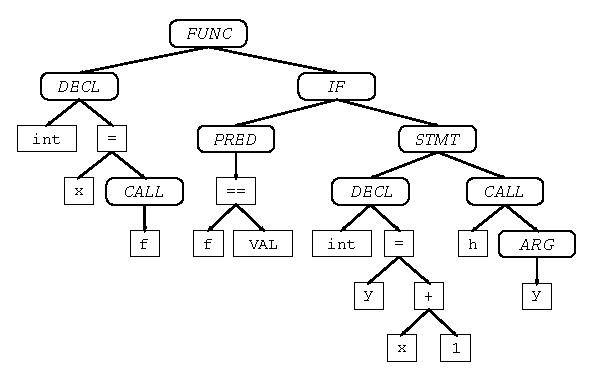
\includegraphics[width=1\textwidth,height=0.65\textwidth,keepaspectratio]{./figure/ast.eps}
		\caption{Abstract Syntax Tree}
		\label{figure:ast}
	\end{subfigure}
	\begin{subfigure}[t]{0.3\textwidth}
		\centering
		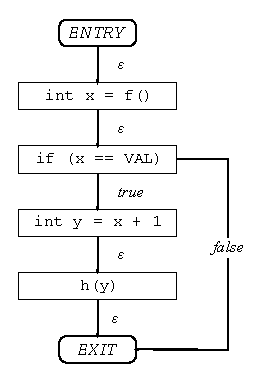
\includegraphics[width=2\textwidth,height=0.65\textwidth,keepaspectratio]{./figure/cfg.eps}
		\caption{Control Flow Graph}
		\label{figure:cfg}
	\end{subfigure}
	\begin{subfigure}[t]{0.3\textwidth}
		\centering
		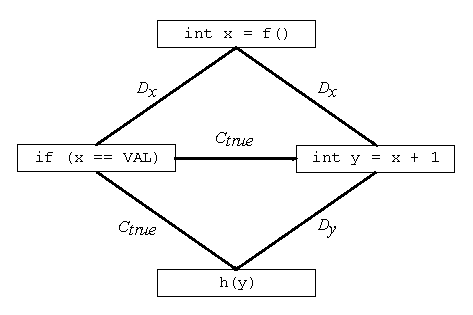
\includegraphics[width=1\textwidth,height=0.65\textwidth,keepaspectratio]{./figure/pdg.eps}
		\caption{Program Dependency Graph}
		\label{figure:pdg}
	\end{subfigure}
	\caption{Representations of code for the example in Figure~\ref{figure:sample}.}
\end{figure*}

\textbf{Abstract Syntax Tree (AST)} Abstract syntax trees represent structure of source code in an abstract way.
Figure~\subref{figure:ast} shows example AST for the code sample Figure~\ref{figure:sample}.
Their nodes do not necessarily correspond to exact syntax token of the program but can represent larger semantic unit such as condition expression or variable declaration.

\textbf{Control Flow Graph (CFG)} Control flow graph describes conditions and order of each execution path of program.
Figure~\subref{figure:cfg} shows example CFG for the code sample given above.
While control flow graph provides information of condition and context, data flow is still required to determine the exact attack vector.

\textbf{Program Dependency Graph (PDG)} Program dependency graph consists of two types of edges: data dependency edges and control dependency edges.
Figure~\subref{figure:pdg} shows example PDG for the code sample given above, data and control dependency edges are labeled as D and C respectively.
Data dependency edges connect variable values and statements affected by them.
Control dependency edges are different from control flow graph since the former do not contain execution order but show dependencies more clearly.

The combination of three graphs forms code property graph shown in Figure~\ref{figure:cpg}.

\subsection{Learning Model for Graph Data}

Since we use code property graph as program representation, we need neural network model which takes graph data as input.
Code property graph is a directed graph with edges of multiple attributes.
We consider typical learning models for graph data:

\textbf{Graph Kernel.} Graph kernel is a function that computes similarities between inputs.
Graph kernel has been mainly applied in bioinformatics and chemoinformatics, for instance, predicting protein function by its structure.
Classical graph kernels are based on walks and paths, subgraphs or subtrees.

Weisfeiler-Lehman (WL) graph kernel \cite{shervashidze2011weisfeiler} is state-of-the-art among graph kernels.
WL graph kernel generates feature vector from subtree pattern in every iteration.
Algorithm first labels each node, and repeates determining subtree pattern from each node.
Feature vector consists of numbers of each label appeared during the algorithm.
The similarity between graphs can be calculated as the inner product of their feature vectors.

\textbf{Graph Neural Network} Graph neural network (GNN) is a learning model which directly uses input graph layout as model \cite{gori2005new}.
GNN extends recursive neural networks, using nodes of input graph as state representations.
For each iteration, state values are updated by being propagating by other connected states.
GNN eventually generates some desired attribute of the input graph.
Li et al. introduced Gated graph sequence neural network (GGS-NN) based on GNN.
GGS-NN is an extend model of GNN which can find the output sequence of graph producing such attribute \cite{li2015gated}.

\textbf{Convolutional Neural Network for Graph} Convolutional neural network (CNN) is typical deep learning model used widely in image recognition.
Typically CNN takes 2-dimensional data, usually image, as input and feed forward them in network with convolution operations.
Niepert et al. presented an approach to process general graphs with CNN by considering input of classical CNN as lattice graph \cite{niepert2016learning}.
From such perspective, receptive field of classical CNN is a neighborhood subgraph from certain node with fixed width.
Thus for an arbitrary input graph, receptive field can be generated and consequenty passed as input to classical CNN.